\section{CAR Model}

\begin{frame}{CAR Model}

\begin{columns}[T,totalwidth=\textwidth]

% ======================================
% LEFT COLUMN (1/3 width)
% ======================================
\column{0.6\textwidth}
\centering
\vspace{0.5cm}
% --- FORMULES (top of left column) ---
{\small Model Formulation with CAR Leroux prior:}
\[
\resizebox{\linewidth}{!}{$
\begin{aligned}
y_i^{\ast}|\alpha,x_i^{\ast},\beta,o_i &\stackrel{\text{ind}}{\sim} \mathcal{N}(\alpha + x_i^{\ast \top} \boldsymbol{\beta} + \phi_i + o_i,\sigma^2),
\quad i= 1,\dots,n \\[0.15cm]
\alpha & \sim \mathcal{N}(0,1000)\\[0.15cm]
\beta & \sim \mathcal{N}(0,1000 \mathrm{I}_p)\\[0.15cm]
%\varepsilon_i &\stackrel{\text{iid}}{\sim} \mathcal{N}(0, \sigma^2), \\[0.25cm]
%\mathbf{\phi} \mid \tau, \rho &\sim \mathrm{CAR}(\tau, \rho, W), \\[0.15cm]
%\phi_i \mid \mathbf{\phi}_{-i}, \tau, \rho
%&\sim
% \mathcal{N}\!\left(
% \frac{\rho}{d_i} \sum_{j \in \mathcal{N}(i)} w_{ij} \phi_j,\;
% \frac{1}{\tau d_i}
% \right),
% & d_i &= \sum_{j} w_{ij}
\phi_i | \phi_{-i},W,\tau^2,\rho &\stackrel{\text{ind}}{\sim} \mathcal{N}\left( \frac{\rho\Sigma_{j=1}^{n}w_{ij}\phi_j}{\rho\Sigma_{j=1}^{n}w_{ij}+1-\rho},\frac{\tau^2}{\rho\Sigma_{j=1}^{n}w_{ij}+1-\rho} \right) \\[0.15cm]
\tau^2 &\sim inv-gamma(1,0.01)\\[0.15cm]
\rho &\sim \mathcal{U}(0,1)
\end{aligned}
$}
\]


% --- SMALL IMAGE (bottom of left column) ---
%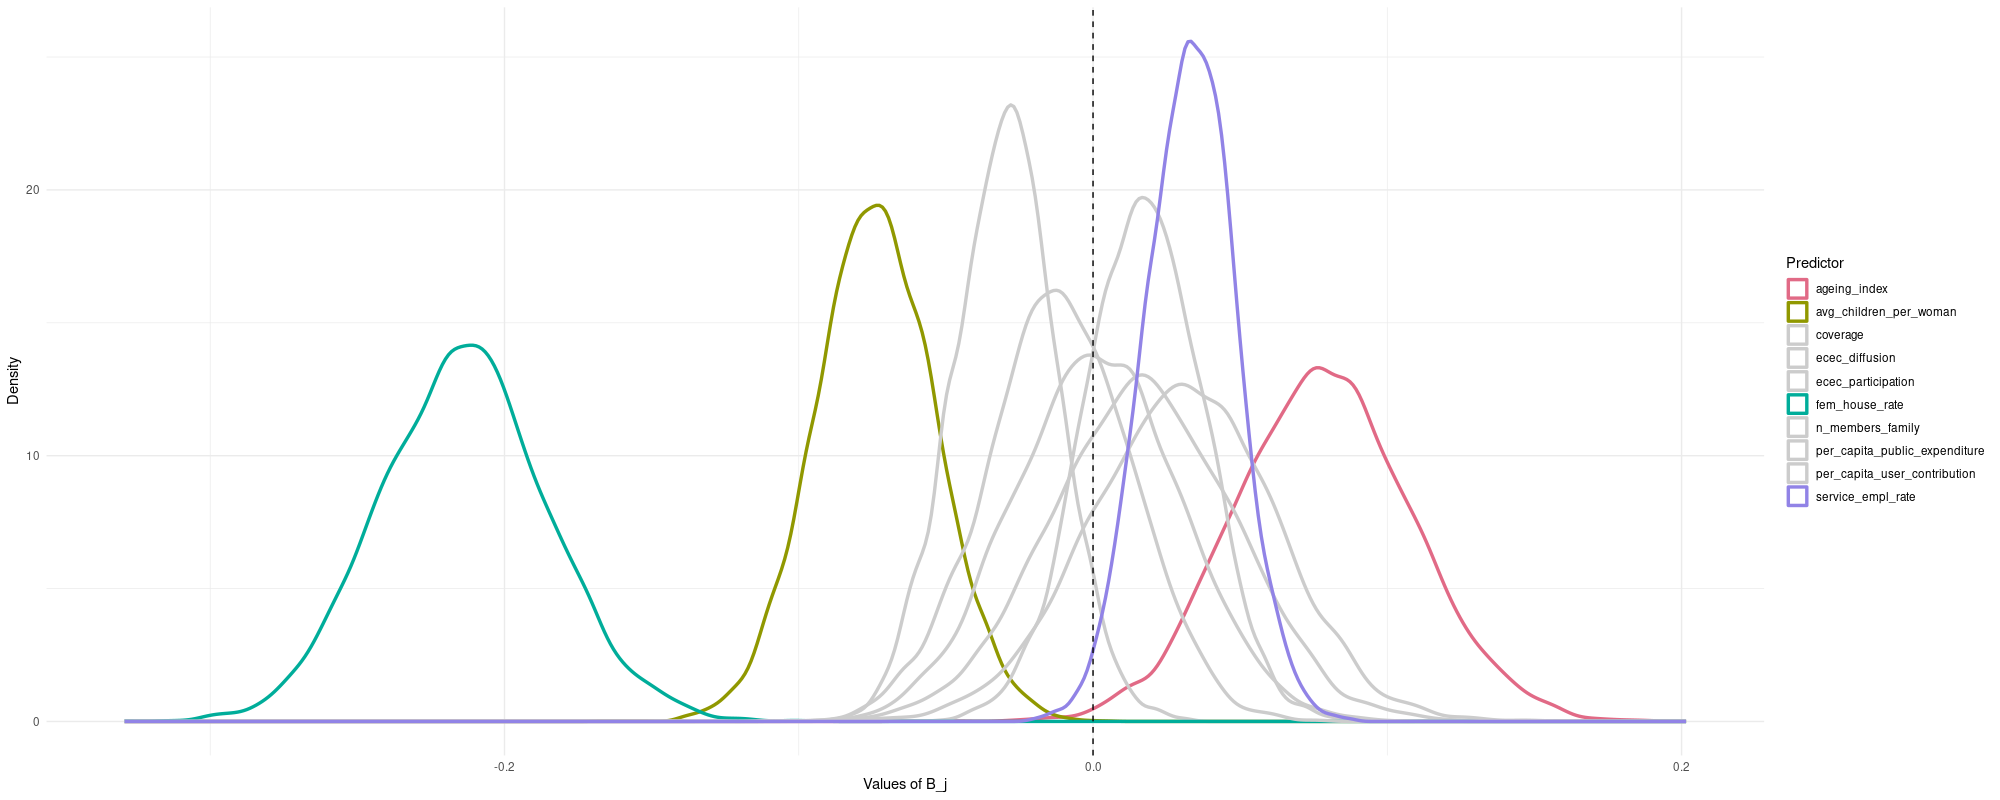
\includegraphics[height=0.4\textheight]{pictures/CAR_beta_posterior.png}

%{\tiny Histograms of Posterior distributions}

% ======================================
% RIGHT COLUMN (2/3 width)
% ======================================
\column{0.45\textwidth}
\centering

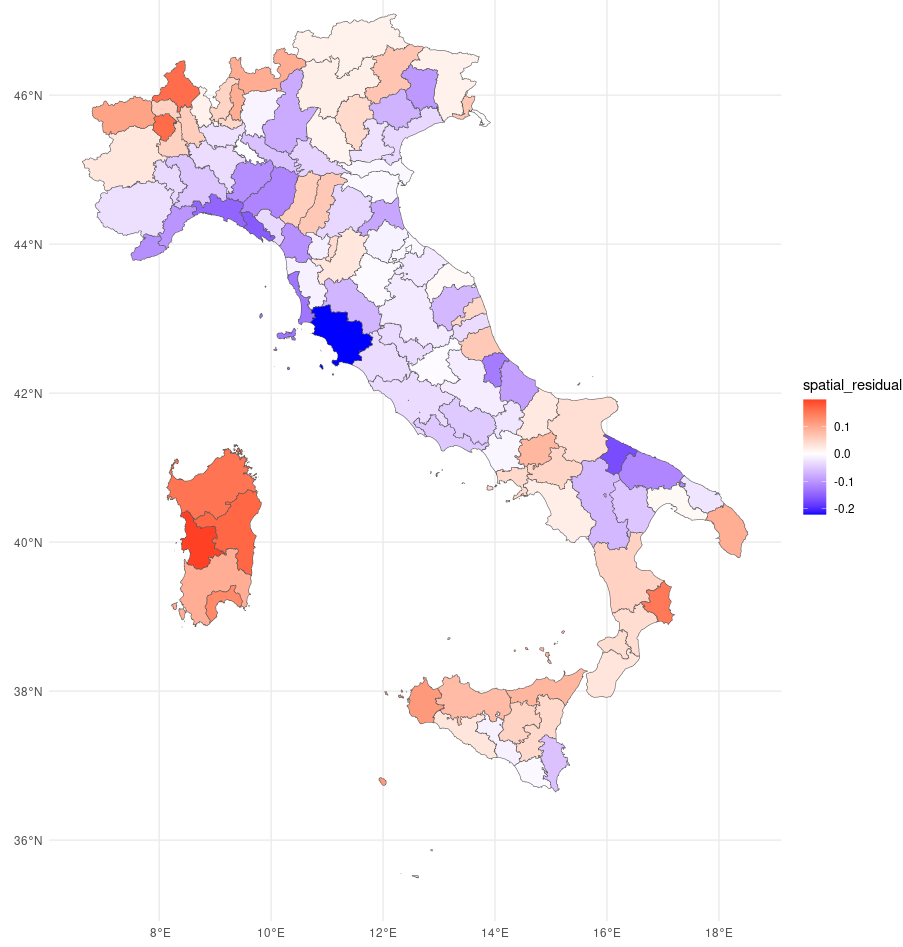
\includegraphics[height=6cm]{pictures/spatial_residuals.png}

{\tiny Posterior Mean of CAR spatial effect}

\end{columns}

\end{frame}

\begin{frame}{CAR model}
\begin{center}
    
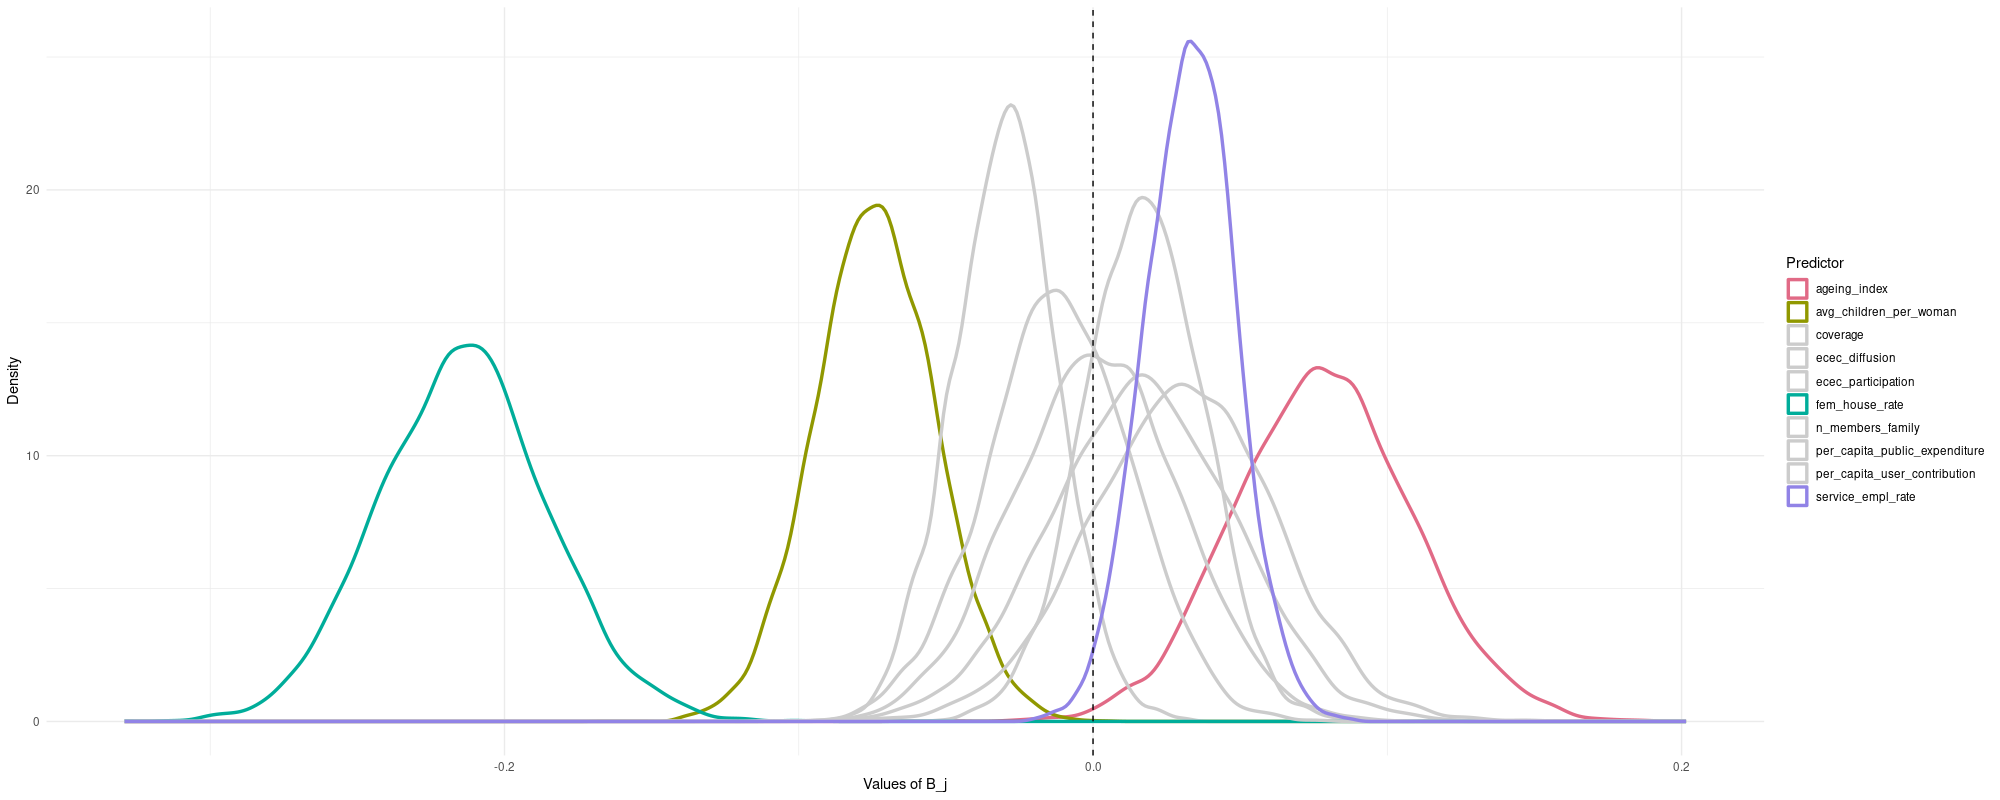
\includegraphics[width=\textwidth, height=0.75\textheight, keepaspectratio]{pictures/CAR_beta_posterior.png}
{\footnotesize Posterior densities of $\beta_j$. The colored densities belong to covariates whose coefficients' 95\% CI does not include zero. Model fitted through CARBayes \cite{carbayes}}
\end{center}    
\end{frame}